\section{Conclusion}
\label{sec:conclusion}

Summing up, this laboratory provided us the opportunity to understand how an audio amplifier circuit works with both its gain and output stages.\par
Similarly to the previous lab assignment, there are some differences between the theoretical and simulation values obtained, this is the case for the OP analysis and also the impedances, for example. This can be explained by the non linear components used in this laboratory: the transistors. In the first 2 lab assignments only linear components were used and because of that the simple theoretical analysis made matched perfectly the simulation analysis, as it should. This was no longer the case in this assignment. \par
As for the merit figure calculation, we used Spice's values as they provide the most accurate results. \par
Finally, we are going to compare the results from simulation and theoretical analysis side by side: \par
%compararações

\begin{center}
  \begin{tabular}{ | c | c | }
    \hline    
    {\bf Name} & {\bf Value} \\ \hline
    \input{m_tab}
  \end{tabular}
  \captionof{figure}{Merit Figure Table}
\end{center}

\begin{center}
  \begin{tabular}{ | c | c | }
    \hline    
    {\bf Name} & {\bf Value [V or A]} \\ \hline
    \input{../mat/OP1}
    \hline
  \end{tabular}
  \captionof{figure}{Theoretical Operating Point Gain Stage}
\end{center}

\begin{center}
  \begin{tabular}{ | c | c | }
    \hline    
    {\bf Name} & {\bf Value [V or A]} \\ \hline
    \input{../mat/OP2}
    \hline
  \end{tabular}
  \captionof{figure}{Theoretical Operating Point Output Stage}
\end{center}

\begin{center}
  \begin{tabular}{ | c | c | }
    \hline    
    {\bf Name} & {\bf Value [V]} \\ \hline
    @g0[i] & -2.62010e-04\\ \hline
@id[current] & 1.039703e-03\\ \hline
@r1[i] & 2.500671e-04\\ \hline
@r2[i] & -2.62010e-04\\ \hline
@r3[i] & -1.19432e-05\\ \hline
@r4[i] & 1.159730e-03\\ \hline
@r5[i] & -1.30171e-03\\ \hline
@r6[i] & 9.096634e-04\\ \hline
@r7[i] & 9.096634e-04\\ \hline
n1 & 5.046111e+00\\ \hline
n2 & 4.787759e+00\\ \hline
n3 & 4.248290e+00\\ \hline
n4 & -1.88445e+00\\ \hline
n5 & 4.824275e+00\\ \hline
n6 & 8.832281e+00\\ \hline
n8 & -2.81232e+00\\ \hline
n9 & -1.88445e+00\\ \hline

  \end{tabular}
  \captionof{figure}{Simulation Operating Point}
\end{center}

\begin{figure}[H]
    \minipage{0.45\textwidth}
      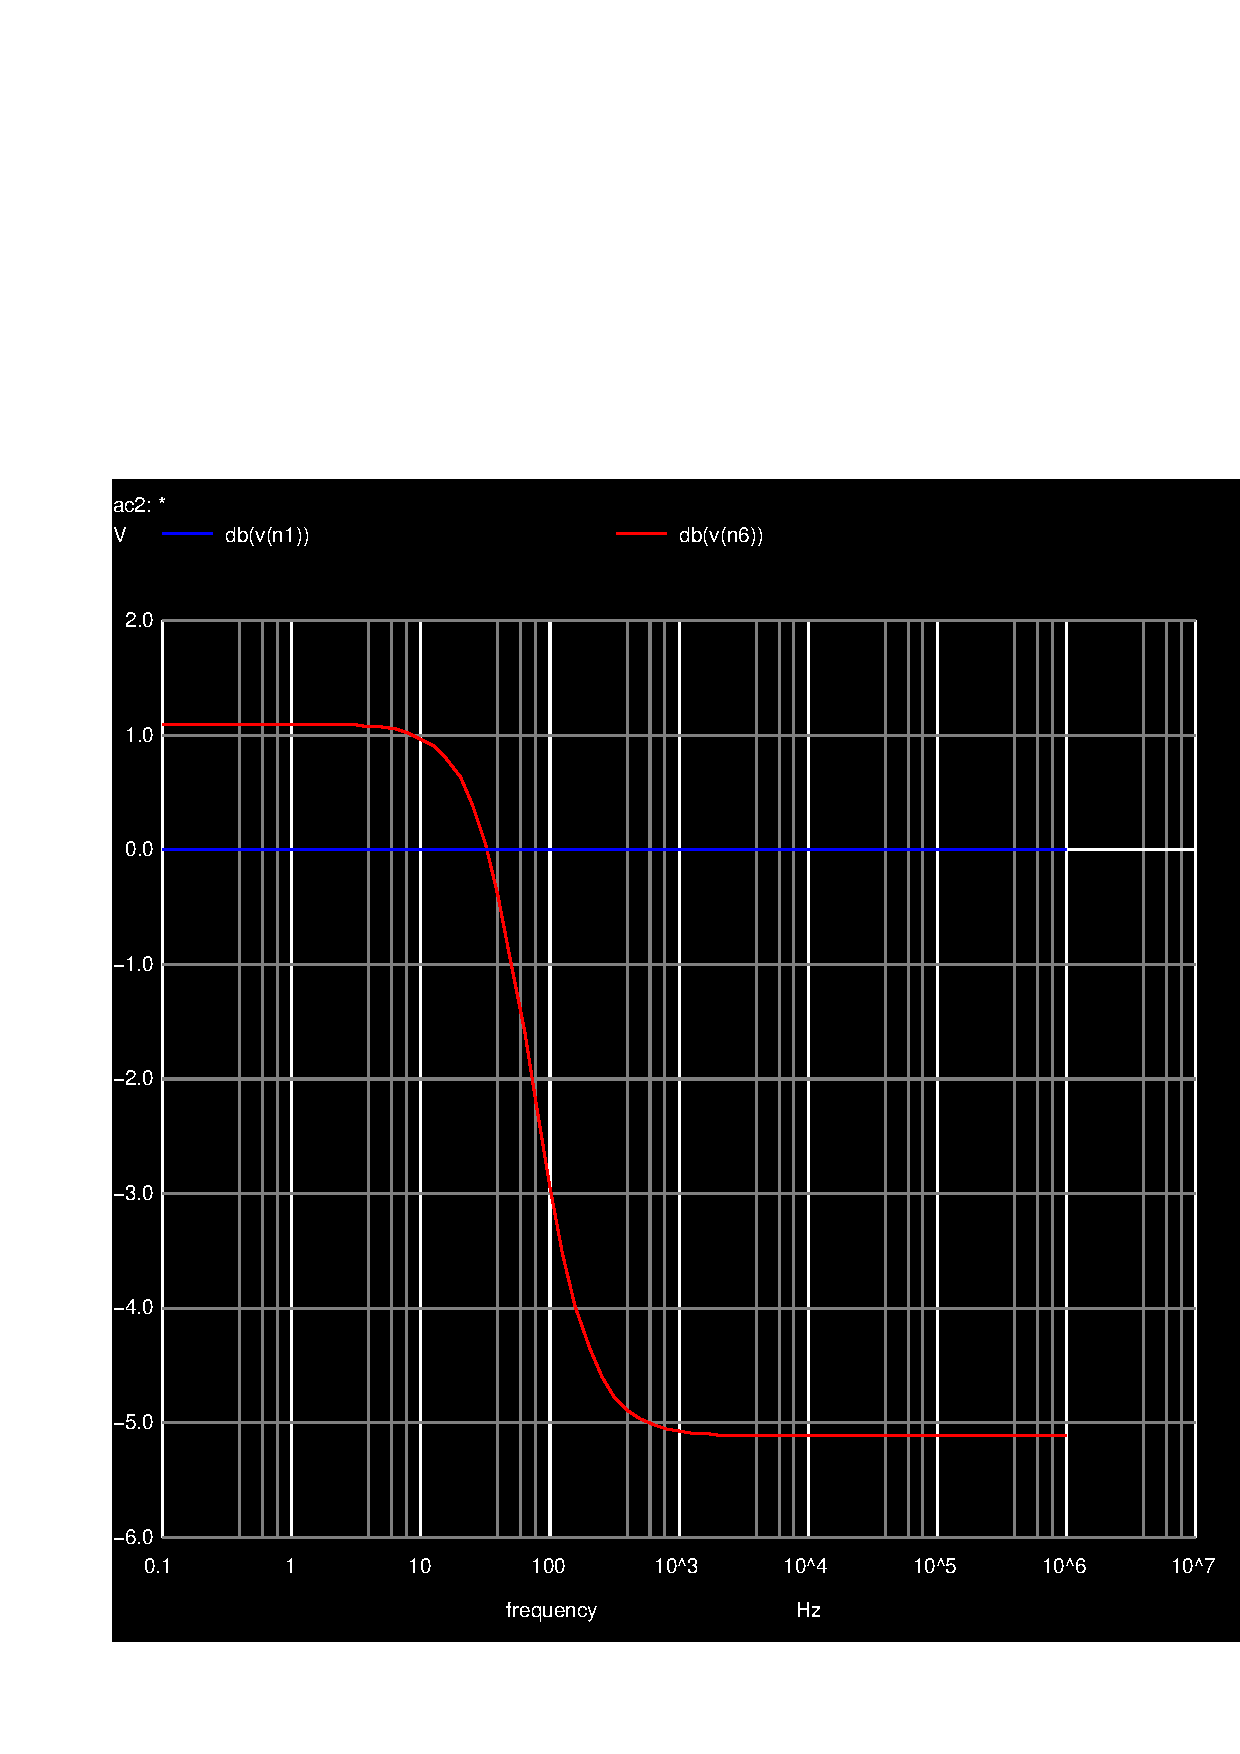
\includegraphics[width=\linewidth]{../mat/fresponse.pdf}
      \caption{Theoretical Gain Frequency Response}
    \endminipage\hfill
    \minipage{0.45\textwidth}
      \includegraphics[width=\linewidth]{../sim/vo2f.pdf}
      \caption{Simulation Gain Frequency Response}
    \endminipage\hfill
\end{figure}

\begin{center}
  \begin{tabular}{ | c | c | }
    \hline    
    {\bf Name} & {\bf Value [$\Omega$]} \\ \hline
    \input{../mat/docImp}
    \hline
  \end{tabular}
  \captionof{figure}{Theoretical Input and Output Impedances}
\end{center}

\begin{center}
  \begin{tabular}{ | c | c | }
    \hline    
    {\bf Name} & {\bf Value [$\Omega$]} \\ \hline
    \input{impedance_tab}
  \end{tabular}
  \captionof{figure}{Simulation Input and Output Impedances}
\end{center}




